\chapter{Benutzeroberfläche}
Die folgenden Darstellungen sollen eine grobe Orientierung für die Benutzeroberflächen des Endprodukts geben. Diese können sich im Verlauf des Projektes noch ändern.
\section{Konfigurations-GUI}
Die Konfigurations-GUI soll einige Optionen bieten, die für reguläre Nutzer des Webinterface nicht verfügbar sein sollte.

\begin{figure}[H]
	\centering
		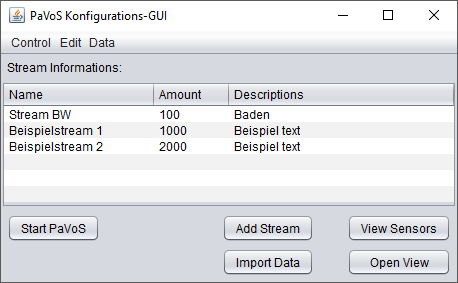
\includegraphics[width=0.6\linewidth]{gui/backend/BackendGUIMain.png}\\
	\caption{Die Konfigurations-GUI zeigt die Streams des Dienstes an. Alle Funktionen sind in den Reitern enthalten. Wichtige Funktionen haben zusätzlich einen Button im unteren Bereich der GUI.}
\end{figure}

\begin{figure}[H]
	\centering
		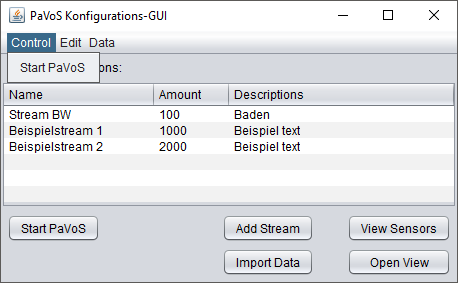
\includegraphics[width=0.6\linewidth]{gui/backend/BackendGUIMenu1.png}\\
	\caption{Control-Reiter: Hier kann der Dienst gestartet und beendet werden.}
\end{figure}

\begin{figure}[H]
	\centering
		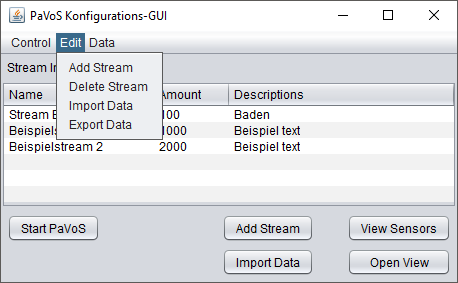
\includegraphics[width=0.6\linewidth]{gui/backend/BackendGUIMenu2.png}\\
	\caption{Edit-Reiter: Dieser Reiter stellt die Funktionen zum hinzufügen oder entfernen der Streams bereit. Außerdem ist es hier möglich Daten zu importieren oder zu exportieren.}
\end{figure}

\begin{figure}[H]
	\centering
		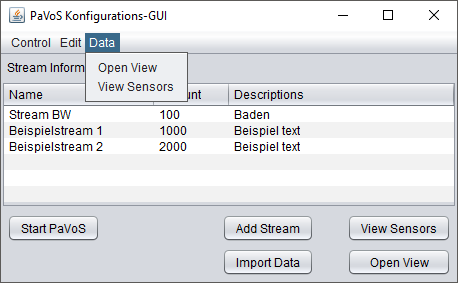
\includegraphics[width=0.6\linewidth]{gui/backend/BackendGUIMenu3.png}\\
	\caption{Data-Reiter: Über den Data-Reiter kann eine Auflistung aller im System enthaltenen Sensoren angezeigt  oder das Webinterface geöffnet werden.}
\end{figure}
\newpage
\section{Webinterface}
Im Folgenden wird das Webinterface des Dienstes vorgestellt. Diese ist in den Grundzügen vergleichbar mit der von \url{maps.luftdaten.info}, bietet jedoch viele zusätzliche Funktionen an.

\begin{figure}[H]
	\centering
		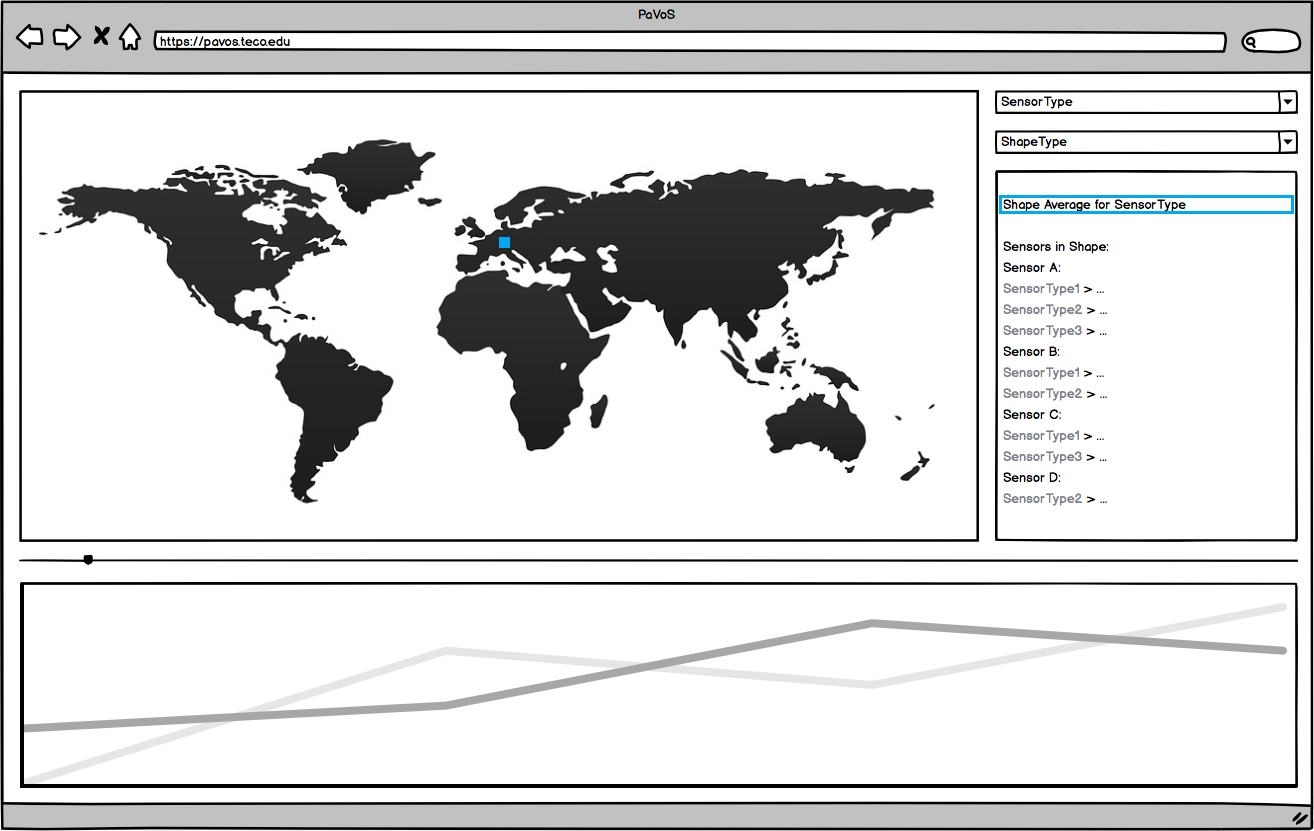
\includegraphics[width=0.9\linewidth]{gui/frontend/FrontGUIWorldWithShapeSelection.png}\\
	\caption{Webinterface mit Weltansicht und ausgewähltem Cluster.\\
	Dies ist der Startpunkt des Dienstes. Von hier aus können alle angebotenen Features bedient werden. Die Karte besteht aus einer Sammlung von Clustern, die - sofern Sensordaten darin enthalten sind - selektiert werden können, um detaillierte Daten einzusehen.\\
	Hier ist auf der Karte ein Cluster selektiert. In der erweiterten Ansicht wird ``Shape Average for SensorType`` ausgewählt, so werden berechnete Durchschnittsdaten in der Detailansicht angezeigt.}
\end{figure}

\begin{figure}[H]
	\centering
		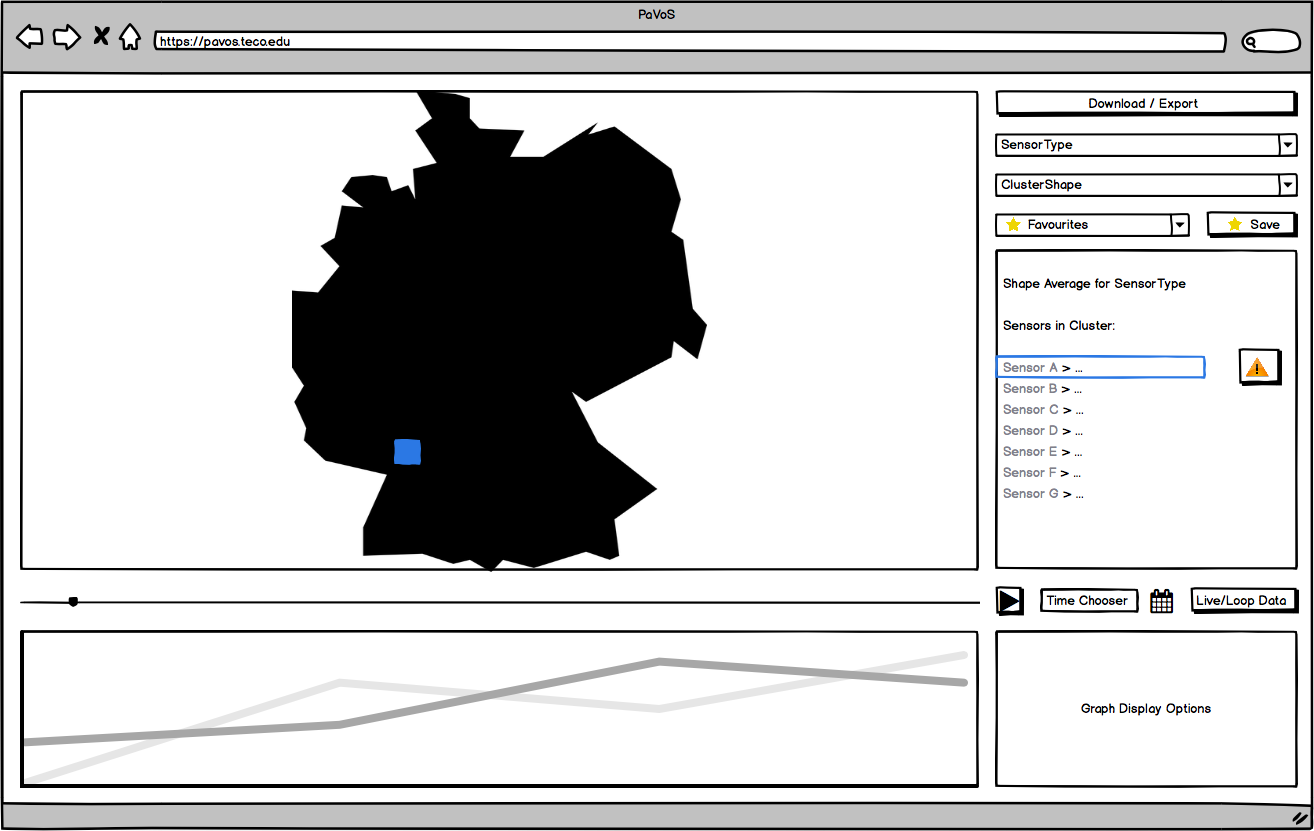
\includegraphics[width=0.9\linewidth]{gui/frontend/FrontGUIGermanyWithShapeSelection.png}\\
	\caption{Webinterface mit Deutschlandansicht und ausgewähltem Cluster.\\
	Hier ist in der erweiterten Ansicht ein bestimmter Sensor selektiert, so werden seine historischen Daten in der Detailansicht angezeigt.}
\end{figure}

\begin{figure}[H]
	\centering
		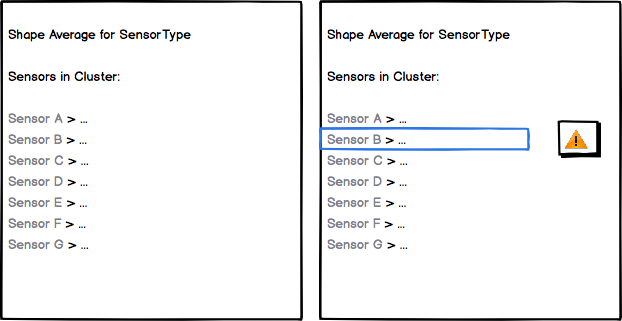
\includegraphics[width=0.8\linewidth]{gui/frontend/FrontGUISensorListAloneAndWithSelection.png}\\
	\caption{Erweiterte Ansicht: Anzeige aller Sensoren innerhalb des ausgewählten Clusters (links). Jeder einzelne Sensor kann ausgewählt werden (rechts), um detaillierte historische Daten anzuzeigen (siehe Detailansicht). Ist ein Sensor ausgewählt, kann er von den Nutzer, unter Angabe eines Grundes, gemeldet werden, indem der Meldebutton genutzt wird (rechts von der Selektion).}
\end{figure}

\begin{figure}[H]
	\centering
	
\includegraphics[width=0.4\linewidth]{gui/frontend/FrontGUISensorType.png}
	\hspace{0.1cm}
	
\includegraphics[width=0.4\linewidth]{gui/frontend/FrontGUIShapeType.png}
	\caption{Dropdown-Listen für den Sensortyp (SensorType) und die Form des Clusters (ClusterShape)}
\end{figure}

\begin{figure}[H]
	\centering
	
\includegraphics[width=0.4\linewidth]{gui/frontend/FrontGUIFavourites.png}
	\caption{Dropdown-Liste für die Favoriten und Button zur Speicherung der derzeitigen Selektion als neuer Favorit.}
\end{figure}

\begin{figure}[H]
	\centering
	
\includegraphics[width=0.4\linewidth]{gui/frontend/FrontGUIDownloadButton.png}\\
	\caption{Downloadbutton zum Export von Daten. Wird der Download angefordert, öffnet sich ein Formular, das die genaue Auswahl der gewünschten Daten ermöglicht.}
\end{figure}

\begin{figure}[H]
	\centering
	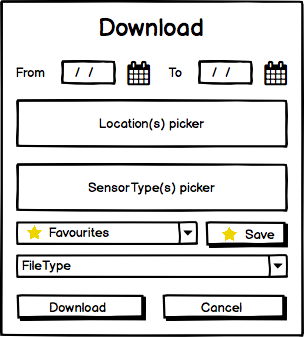
\includegraphics[width=0.5\linewidth]{gui/frontend/FrontGUIExportForm.png}\\
	\caption{Downloadformular zum Export von Daten. Wird der Download angefordert, wird immer zuerst der Download der derzeit ausgewählten Daten angeboten. Das Formular ermöglicht es dem Nutzer den Download nach Zeitintervallen, Lokalitäten und Sensortypen auf seine Bedürfnisse anzupassen. Alternativ können auch gespeicherte Favoriten ausgewählt, oder neue gespeichert werden.}
\end{figure}
\newpage
\begin{figure}[H]
	\centering
	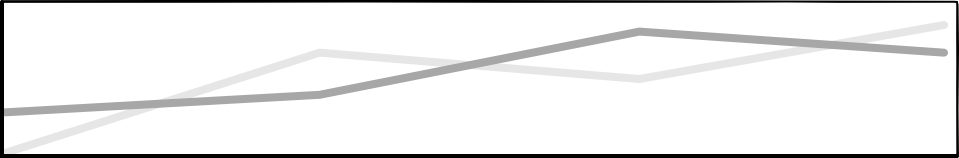
\includegraphics[height=1.5cm]{gui/frontend/FrontGUIDetailGraph.png}
	\hspace{0.1cm}
	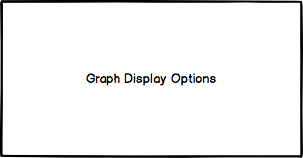
\includegraphics[height=1.5cm]{gui/frontend/FrontGUIGraphSettings.png}
	\caption{Detailansicht: zeitlicher Verlauf spezifischer Sensordaten (Kann ein einzelner Sensor sein, oder der Schnitt eines Clusters). Zusätzlich können rechts Anzeigeoptionen für den Graphen eingestellt werden.}
\end{figure}

\begin{figure}[H]
	\centering
	
\includegraphics[width=0.69\linewidth]{gui/frontend/FrontGUITimeSlider.png}
	\hspace{0.1cm}
	
\includegraphics[width=0.21\linewidth]{gui/frontend/FrontGUITimeSetter.png}
	\caption{Der Zeitregler dient dazu, historische Daten auf der Karte und der erweiterten Ansicht anzuzeigen. Befindet man sich in der Liveansicht, kann man in einen Loop wechseln, der historische Daten in einer Schleife anzeigt. Dieser kann mit dem Play/Pause Button jederzeit unterbrochen oder fortgesetzt werden. Es ist ebenfalls möglich einen gewünschten Zeitpunkt direkt einzugeben. Mit dem Liveansicht-Button kann jederzeit in wieder auf Livedaten gewechselt werden.}
\end{figure}
\newpage
\begin{figure}[H]
	\centering
	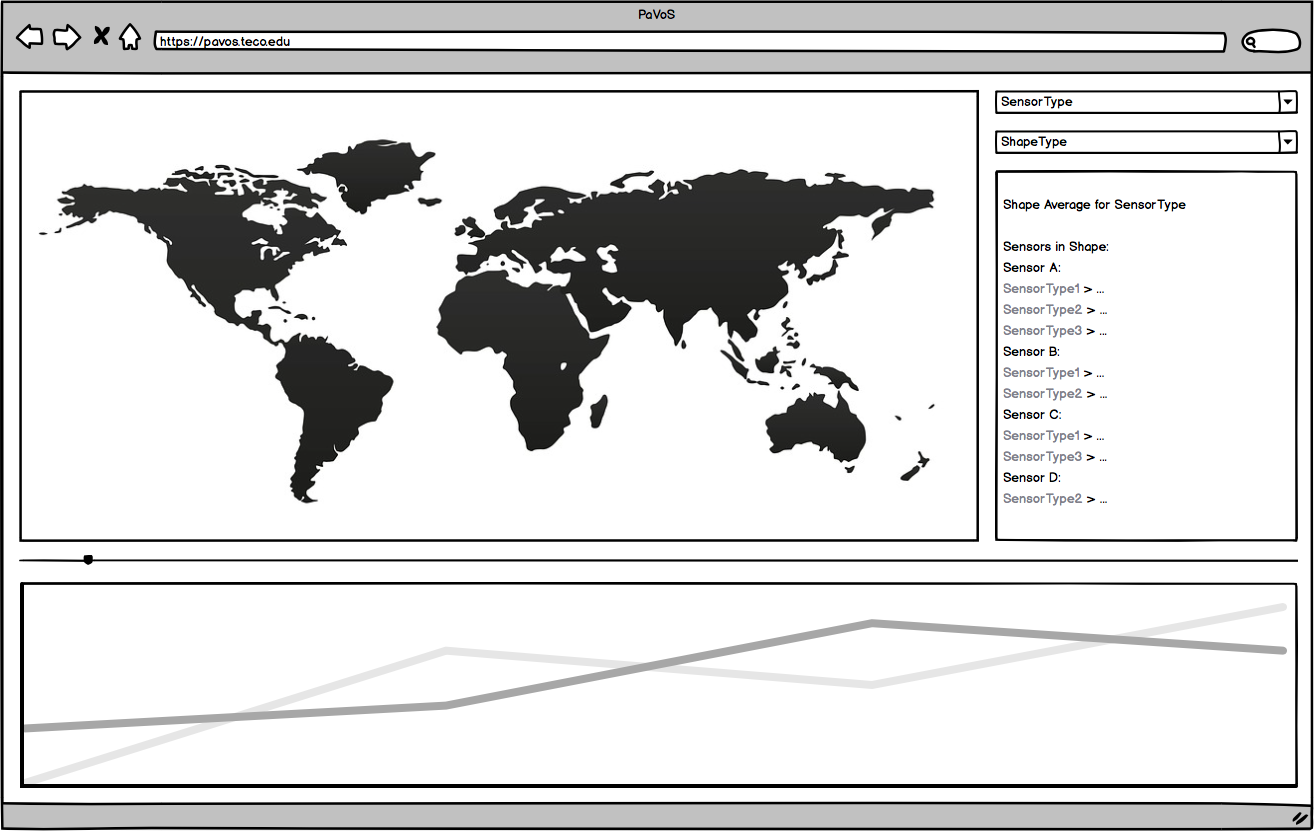
\includegraphics[height=\linewidth, angle=90]{gui/frontend/FrontGUIWorld.png}\\
	\caption{Großansicht Webinterface mit Weltkarte}
\end{figure}